\documentclass[border=0.2cm]{standalone}
\usepackage{pgfplotstable}
\usepackage{pgfplots}
\usepackage{filecontents}


\begin{document}

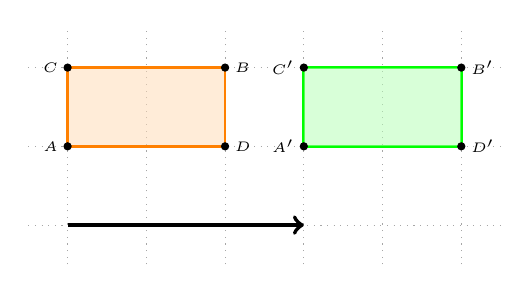
\begin{tikzpicture}

\draw[step=1,gray!70,dotted] (-.5,-1.5) grid (5.5,1.5);

\fill[orange!30,opacity=0.5] (0,0) rectangle (2,1);
\draw[line width=1pt, orange] (0,0) rectangle (2,1);

\draw[line width=1pt, green] (3,0) rectangle (5,1);
\fill[green!30,opacity=0.5] (3,0) rectangle (5,1);

\draw[line width=1.5pt,->] (0,-1) -- (3,-1);

\fill (0,0) circle (1.5pt) node[left] {\tiny $A$};
\fill (2,1) circle (1.5pt) node[right] {\tiny $B$};
\fill (0,1) circle (1.5pt) node[left] {\tiny $C$};
\fill (2,0) circle (1.5pt) node[right] {\tiny $D$};

\fill (3,0) circle (1.5pt) node[left] {\tiny $A'$};
\fill (5,1) circle (1.5pt) node[right] {\tiny $B'$};
\fill (3,1) circle (1.5pt) node[left] {\tiny $C'$};
\fill (5,0) circle (1.5pt) node[right] {\tiny $D'$};


\end{tikzpicture}

\end{document}